\section{Runtime}
\label{section:noderuntime}

We define the session runtime for the \trole{Svr} endpoint
of the \tprotocol{Adder} protocol in Svr.ts,
named after the endpoint.
It exposes a \textbf{public API}
with seams for the developer to pass in the WebSocket server 
and application logic
(i.e. their handler implementations).
It is developer's responsibility to construct the
WebSocket server and set it up to listen for incoming connections.
Internally, it keeps a \textit{private API}
for executing the EFSM, when all participants have 
joined the session.

\begin{lstlisting}[language=javascript]
export class Svr {
	constructor(wss: WebSocket.Server,
				initialState: Implementation.S51) { ... }
	...
}

// Not exported to developer
class Session {
	private wss: WebSocket.Server;
	private initialState: Implementation.S51;
	private roleToSocket: RoleToSocket;
	...
}
\end{lstlisting}

The role of the public API is to manage incoming connections and
wait for all participants to join the session 
(\cref{subsection:noderuntimepublic}), before
handing off to the private API to execute the EFSM
(\cref{subsection:noderuntimeprivate}).

\subsection{Managing Connections}
\label{subsection:noderuntimepublic}

The constructor of the public API class sets up
the framework for mapping incoming WebSocket connections to
participants. 
The main challenge is to wait for all participants to 
connect to the server endpoint before EFSM execution begins.
We address this by defining an internal protocol for managing
session joining -- since we generate the runtime for both server 
and browser endpoints, we can implement this in a way that is 
transparent to the developer.

\begin{figure}[!h]
\begin{lstlisting}[language=javascript,tabsize=2]
const waiting: Set<Roles.Peers> = new Set([Roles.Peers.Client]); (*@\label{line:initwaiting}@*)

const roleToSocket: Partial<RoleToSocket> = { (*@\label{line:initroletosocket}@*)
	[Roles.Peers.Client]: undefined,
};

const onSubscribe = ({ data, target: socket }) => {
	const { connect: role } = JSON.parse(data) 
		as Message.ConnectRequest; (*@\label{line:connectionrequest}@*)
	if (!waiting.has(role)) { return socket.close(); } (*@\label{line:occupied}@*)
	
	roleToSocket[role] = socket; (*@\label{line:connectwsbind}@*)
	waiting.delete(role);
	
	if (waiting.size === 0)
		new Session(wss, roleToSocket as RoleToSocket, initialState); (*@\label{line:newsession}@*)
};

wss.addEventListener('connection', ws => {
	ws.onmessage = onSubscribe; (*@\label{line:wslisteneroverride}@*)
});
\end{lstlisting}
\captionof{lstlisting}{Handling Connections in Server Endpoint}
\label{lst:nodeconnect}
\end{figure}

We show this in \cref{lst:nodeconnect} and walk through
the main parts:

\begin{enumerate}
\item
The server keeps track of the participants that 
have yet to join the session -- this is initialised to the
complete set of
non-server endpoints at the start (\cref{line:initwaiting}).

\item
Browser endpoints request to join the session
by sending a \textit{connection request} with the role
identifier as payload (\cref{line:connectionrequest}). 
We generate role enums for browser targets
in the same way, so the server can correctly
interpret the message.
We listen to connection requests by overriding the
\texttt{onmessage} event listener for every new connection
(\cref{line:wslisteneroverride}).

\item
If the role is already occupied, then the server
responds by closing the connection (\cref{line:occupied}).

\item
Otherwise, the role is not occupied, so the server binds
the WebSocket (which the message was received from) to the role
(\cref{line:connectwsbind}).
This is accumulated in an interface type, mapping each
role to an \textit{optional}\footnote{
TypeScript provides utility types for common type transformations:
\texttt{Partial<T>} constructs a type with all properties
of \texttt{T} set to optional.
} 
WebSocket property
-- for roles who have
not yet connected, we do not know the WebSocket binding, so the
WebSocket for these roles are \lstonelinejs{undefined},
as initialised at the start (\cref{line:initroletosocket}).

\item
When the server is no longer waiting for any participants,
it notifies all other roles through the bounded WebSocket
connections that the session will start, and delegates
EFSM execution to the private API by constructing
an instance of the \texttt{Session} class (\cref{line:newsession}).
The notification process is managed by the \texttt{Session} class.

\begin{lstlisting}[language=javascript,tabsize=2,numbers=none]
Object.values(roleToSocket).forEach(socket => {
	socket.send(JSON.stringify(Message.ConnectConfirm));
});
\end{lstlisting}

\item
We define the interfaces and factories for connection messages 
in the generated EFSM.ts file under
the \texttt{Message} namespace.

\begin{lstlisting}[language=javascript,tabsize=2,numbers=none]
// Inside the Message namespace...
export interface ConnectRequest { connect: Role.Peers };
export const ConnectConfirm = { connected: true };
\end{lstlisting}
\end{enumerate}

\subsection{Executing the EFSM}
\label{subsection:noderuntimeprivate}

The \texttt{Session} class executes the EFSM.
We define a transition function, \texttt{next()}, 
parameterised by the current state,
The constructor of the \texttt{Session} class
explicitly calls \texttt{next()} with the 
initial state implementation provided by the developer
to start EFSM execution.
\texttt{next()} invokes the handler defined by the developer
and performs the required channel actions for non-terminal states.

\begin{itemize}
\item 
For \textbf{send} states, the handler will
return the label and payload to be sent, along with the
successor state implementation. The transition function
should construct and send the message, 
and transition to the successor state.

\item
For \textbf{receive} states, we change the
message event listener on the WebSocket to
pass the incoming message to the handler.
The handler will return the successor state,
which the runtime can transition to.

\end{itemize}

We conceptualise this in \cref{lst:noderuntimesimple}.
The discriminated union lets the runtime figure out
the type of the current state.

\begin{figure}[!h]
\begin{lstlisting}[language=javascript,tabsize=2]
next(state: Implementation.Type) {
	switch (state.type) {
		case 'Send': {
			const [label, payload, succ]: (*@\hl{???}@*) = state.handler;	 (*@\label{line:noderuntimebadtype1}@*)
			this.send((*@\hl{???}@*), label, payload); (*@\label{line:noderuntimeunknownrole}@*)		
			return this.next(succ);
		}
		case 'Receive': {
			this.wss.onmessage = ({ data }) => {
				const { label, payload } = JSON.parse(data) as (*@\hl{???}@*); (*@\label{line:noderuntimebadtype2}@*)
				const succ: (*@\hl{???}@*) = state.handler[label](...payload); (*@\label{line:noderuntimebadtype3}@*)
				return this.next(succ);
			}
		}
		case 'Terminate': { return; }
	}
}
\end{lstlisting}
\captionof{lstlisting}{Conceptual EFSM Transition Function 
for Server-Side Endpoint}
\label{lst:noderuntimesimple}
\end{figure}

However, we still face problems with resolving types, as highlighted.
Just because we know that the current state is a send state,
we do not know \textit{which} particular state it is,
so we cannot accurately type the handler (\cref{line:noderuntimebadtype1}).
The same problem is amplified for the receive state:
we need to know the specific receive state in order
to correctly serialise the message (\cref{line:noderuntimebadtype2})
and interpret the successor state (\cref{line:noderuntimebadtype3}).
We see another problem with handling send states:
because we do not know the specific send state, we do not know which
participant to send the message to (\cref{line:noderuntimeunknownrole}).

\begin{figure}[!h]
\begin{lstlisting}[language=javascript,tabsize=2]
abstract class ISend {
	type: 'Send' = 'Send';
	abstract performSend(
		next: EfsmTransitionHandler,
		send: (role: Roles.Peers, label: string, payload: any[]) 
			=> void,
	): void;
};

abstract class IReceive {
	type: 'Receive' = 'Receive';
	abstract prepareReceive(
		next: EfsmTransitionHandler,
		register: (from: Roles.Peers, messageHandler: MessageHandler)
			=> void,
	): void;
};
\end{lstlisting}
\captionof{lstlisting}{Class Definitions for \texttt{Implementation} API}
\label{lst:nodeabstractclass}
\end{figure}

These all reduce to the same core problem: the runtime
needs to know the specific state at compile-time\footnote{
Whether TypeScript ``compiles'' or ``transpiles''
(or even \textit{``transcompiles''} \cite{transcompiles}) to JavaScript
is not relevant to our work; we stick with compilation
and keep our terminology consistent.}.
We solve this through \textit{runtime polymorphism} instead, since
the specific type of \texttt{state} is known at runtime.
For each type of state, we define a common API that can be invoked
by the EFSM transition function. To achieve runtime polymorphism,
each concrete state must provide a specific implementation: 
this motivates our design for defining the discriminated union
using abstract classes with abstract methods 
(\cref{lst:nodeabstractclass}).

\begin{figure}[!h]
\begin{lstlisting}[language=javascript,tabsize=2]
next(state: Implementation.Type) {
	switch (state.type) {
		case 'Send':
			return state.performSend(this.next, this.send);
		case 'Receive':
			return state.prepareReceive(this.next, this.register);
		case 'Terminal':
			return;
	}
}
\end{lstlisting}
\captionof{lstlisting}{Final EFSM Transition Function for Server-Side
Endpoint}
\label{lst:noderuntime}
\end{figure}

Using this approach,
we can pass the transition function and channel actions 
from the \texttt{Session} runtime class
to the individual state \texttt{Implementation} classes:
these are also generated by \fancyname{NodeTS}, so we
guarantee linear usage of channel resources by construction as well.
This \textit{significantly} simplifies the design of the runtime
(\cref{lst:noderuntime}),
because the transition function no longer needs to know the type 
of the specific state at compile-time.

By passing the specific functions defined in the runtime
to the individual EFSM states, we can visualise our runtime
as a \textit{message passing} abstraction 
(\cref{fig:noderuntimeefsm}): the runtime uses the common
\texttt{performSend()} or \texttt{prepareReceive()} API
to delegate to the specialised implementation, which will in turn
ask the runtime to perform specialised channel actions using
the parameterised methods, and finally delegate back to
the runtime to transition to the specific successor state.

\begin{remark}
We need to be careful when passing \textit{instance} methods
as \textit{function} arguments 
-- namely, the semantics of \lstonelinejs{this} is different.
In short, we have to \textit{explicitly}
\texttt{bind()} the \texttt{Session} object
to the instance methods that we pass as function arguments:

\begin{lstlisting}[language=javascript,tabsize=2]
// Inside the Session class constructor...
this.next = this.next.bind(this);
this.send = this.send.bind(this);
this.register = this.register.bind(this);
\end{lstlisting}

Not doing so will result in \lstonelinejs{this} taking
a different value 
(either the global object or \lstonelinejs{undefined}).
\end{remark}

We elaborate on how this mechanism
handles the sending and receiving of messages in
\cref{subsection:noderuntimesend,subsection:noderuntimereceive}
respectively.

\begin{figure}[!ht]
\centering
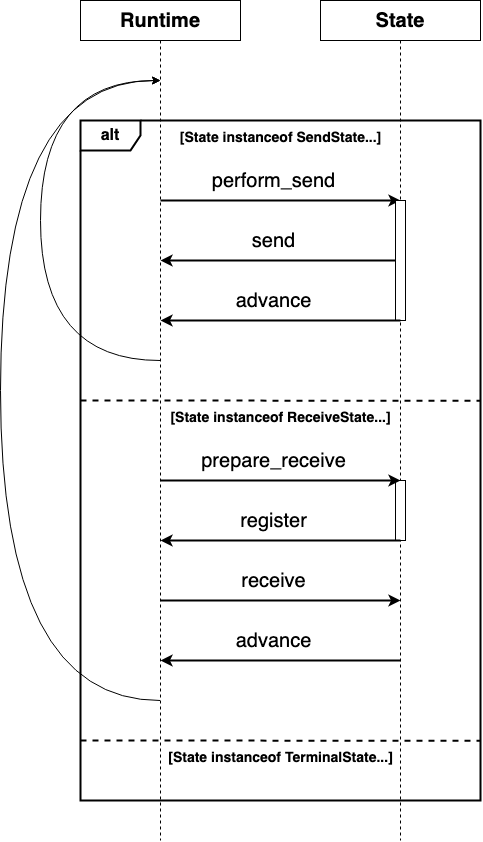
\includegraphics[width=0.5\textwidth]{NodeRuntimeEFSM}
\captionof{figure}{``Message Passing'' Abstraction of EFSM Execution for
Server Endpoints}
\label{fig:noderuntimeefsm}
\end{figure}

\subsection{Sending Messages}
\label{subsection:noderuntimesend}

This is rather straightforward: 
we show the generated code in \cref{lst:nodesend}.

\begin{figure}[!h]
\begin{lstlisting}[language=javascript,tabsize=2]
export class S54 extends ISend {
	constructor(private handler: Handler.S54) { super(); }

	performSend(
		next: EfsmTransitionHandler,
		send: (role: Roles.Peers, label: string, payload: any[]) 
			=> void
	) {
		const [label, payload, successor] = this.handler;
		send(Roles.Peers.Client, label, payload); (*@\label{line:nodesendrole}@*)
		return next(successor);
	}
}
\end{lstlisting}
\captionof{lstlisting}{Generated Code for \texttt{Implementation} API for
Send State}
\label{lst:nodesend}
\end{figure}

We get the label, payload and successor implementation
directly from the handler implemented by the developer, 
accurately typed by how we define the handler API in EFSM.ts.
The developer does not need to specify which role
to send to: this is a sensible design choice, as we know this
from the Scribble protocol, so we do not need the developer 
to specify separately.
As a result, we generate the code to send the message
to the correct role (\cref{line:nodesendrole}).
We use the \texttt{send()} method passed down
by the runtime to commit our communication action:
the runtime will handle how to serialise the message and perform
the send. We guarantee that \texttt{send()} is called
\textbf{exactly once} by construction, thus channel linearity
is never violated.
Finally, we use the parameterised EFSM transition handler
to notify the rutime which specific state to transition to.

\subparagraph{Sending through WebSockets}
We define message structures as interfaces, which
are represented by objects. 
By convention in \fancyname{SessionTS},
we serialise messages into \textit{JavaScript Object Notation}
(or JSON) \cite{json} using the built-in \texttt{JSON.stringify()}
method.

\begin{lstlisting}[language=javascript]
send(role: Roles.Peers, label: string, payload: any[]) {
	this.roleToSocket[role].send(JSON.stringify({
		label, payload
	});
}
\end{lstlisting}

They are decoded using the same interface schema on the receiving end
using \texttt{JSON.parse()}: whilst the method return type is the
dynamic \lstonelinejs{any} type, 
we guarantee type safety by construction
as we performed the serialisation in the first place, so
we can safely interpret the deserialised content 
using a concrete type.

\subsection{Receiving Messages}
\label{subsection:noderuntimereceive}

We need to update the message event listener on the WebSocket
to use the developer's handler -- 
specific to the \textit{current state} -- 
to process the message.
Our approach is to keep the WebSocket message event listener
untouched, but define it in a way that allows \textit{dynamic} behaviour.
We walk through the concept implemented in (\cref{lst:noderuntimewsmsg}):

\begin{enumerate}
\item 
\texttt{Session} keeps track of the \textit{current}
message receive handler (\cref{line:noderuntimehandler}).
The \texttt{?} syntax denotes it is an \textit{optional}
type: not every state is a receive state, so there does not \textit{have} to
be an active message handler.

\item
The receive handler does \textit{not} need a specialised type
(\cref{line:msghandler}). The receive handler is defined in
the \texttt{Implementation} class of the concrete receive state,
so it will deserialise the message to the correct form.

\item
The \texttt{register()} method (\cref{line:register})
is passed to the \texttt{Implementation} class of the concrete
receive state, which will construct the message handler
around the developer's handler implementation and register it
with the runtime.

\item
When a message is received from the channel,
we dynamically process it with 
the current registered handler (\cref{line:callhandler}).
We encapsulate this dynamic behaviour in an instance method
and bind it as an event listener (\cref{line:wsbind})
for the WebSocket connection
of each non-server endpoint.
\end{enumerate}

\begin{figure}[!h]
\begin{lstlisting}[language=javascript,tabsize=2]
type MessageHandler = (message: any) => void; (*@\label{line:msghandler}@*)

class Session {
	private handler?: MessageHandler; (*@\label{line:noderuntimehandler}@*)

	constructor(...) {
		...
		Object.values(this.roleToSocket).
			.forEach(ws => ws.onmessage = this.receive.bind(this)); (*@\label{line:wsbind}@*)
		this.handler = undefined;
	}
	
	register(handler: MessageHandler) { this.handler = handler; } (*@\label{line:register}@*)

	receive({ data }: WebSocketMessage) {
		const handler = this.handler; (*@\label{line:callhandlerstart}@*)
		this.handler = undefined; (*@\label{line:callhandler2}@*)
		handler?.(data); (*@\label{line:callhandler}@*)
	}
}
\end{lstlisting}
\captionof{lstlisting}{Approach to Dynamic WebSocket Message Event Listener}
\label{lst:noderuntimewsmsg}
\end{figure}

We also show the generated code for the \texttt{Implementation}
class of the receive state in \cref{lst:nodereceive}
-- this should appear consistent
with the explanation above.

\begin{figure}[!h]
\begin{lstlisting}[language=javascript,tabsize=2]
export class S51 extends IReceive {
	
	constructor(private handler: Handler.S51) { super(); }

	prepareReceive(
		next: EfsmTransitionHandler,
		register: (from: Roles.Peers, messageHandler: MessageHandler)
			=> void
	) {
		const messageHandler = (message: any) => {
			const decoded = JSON.parse(message) as Message.S51;
			switch (decoded.label) {
				case Labels.S51.ADD: {
					const successor = 
						this.handler[decoded.label](...decoded.payload);
					return next(successor);
				}
				case Labels.S51.QUIT: {
					const successor = 
						this.handler[decoded.label](...decoded.payload);
					return next(successor);	
				}
			}            
		}
		register(Roles.Peers.Client, messageHandler);
	}
}
\end{lstlisting}
\captionof{lstlisting}{Generated Code for \texttt{Implementation} API for
Receive State}
\label{lst:nodereceive}
\end{figure}

Ideally, a more succinct (and direct) representation would be
\begin{lstlisting}[language=javascript]
(message: any) => {
	const decoded = JSON.parse(message) as Message.S51;
	const successor = 
		this.handler[decoded.label](...decoded.payload);
	return next(successor);
}
\end{lstlisting}

But this expresses a type dependency between \texttt{label}
and \texttt{payload} which, as discussed 
(\cref{subsubsection:dependenttypes}), cannot be implemented.
However message structures \textit{precisely} 
define a discriminated union 
(the label acts as the discriminant 
to distinguish between payload types),
so we handle this with a switch statement,
at the cost of having the same code in each case --
TypeScript does infer the correct specific type in each case statement,
so code duplication here does serve a functional purpose.

Returning to \cref{lst:noderuntimewsmsg},
note that the type of the \texttt{handler} property is \textit{optional}
-- this hints at a problem: 
\textit{how do we know that \texttt{this.handler} is set when
a message is received?} The types imply that we \textit{do not},
and this is indeed the case.
In fact, when we consider a \textit{multiparty} context,
our approach with receive handler registration 
using an optional value actually \textit{fails} to guarantee correctness.
We motivate the problem with a worked
example.

\begin{example}[``Out-of-order'' message receives]
Recall that Node.js is a single-threaded event loop runtime, so
when a message arrives, 
the \texttt{onmessage} event is \textit{queued},
and current execution is \textit{not pre-empted}.

Now consider a multiparty session specified by the global type

\[
A \to S: \text{\lstonelinejs{M1(string)}}. 
B \to S: \text{\lstonelinejs{M2(number)}}. \texttt{end} 
\]

Suppose \trole{S} is the server endpoint.
We describe a possible execution flow for the protocol
that breaks our implementation:

\begin{enumerate}
\item 
\trole{S} transitions to its initial state, 
``receive \lstonelinejs{M1(string)} from \trole{A}''.
The receive handler for \tmsg{M1} is registered.

\item
\tmsg{M2} arrives at \trole{S}, so the \texttt{onmessage} handler
is queued. This is \textit{perfectly plausible}: there
is no causal relation between \tmsg{M1} and \tmsg{M2}.

\item
\tmsg{M1} arrives at \trole{S}, so the \texttt{onmessage} handler
is queued.

\item
The \texttt{onmessage} handler for \tmsg{M2} is executed.
The registered handler expects \lstonelinejs{M1(string)},
but it is called with \lstonelinejs{M2(number)}, which raises
a runtime type error.
\end{enumerate}

This exposes a problem: 
the order of message \textit{arrivals} may not
correspond with the order of \textit{receiving} messages as
specified in the protocol,
\textit{so} the message may arrive before its
corresponding handler is registered.
\end{example}

We observe that message arrivals do not have to be causally related.
However, if we consider a similar \textit{binary} example
\[
A \to S: \text{\lstonelinejs{M1(string)}}. 
A \to S: \text{\lstonelinejs{M2(number)}}. \texttt{end}
\]
then \tmsg{M1} \textit{must} arrive before \textit{M2},
since this is sent through the WebSocket connection between 
\trole{A} and \trole{S}, and FIFO guarantees are respected 
for each individual WebSocket connection. 
We visualise the possible orders of message receive events
in \cref{fig:nodereceivecompare}.

\begin{figure}[!h]
\centering
\begin{subfigure}[b]{0.8\textwidth}
\centering
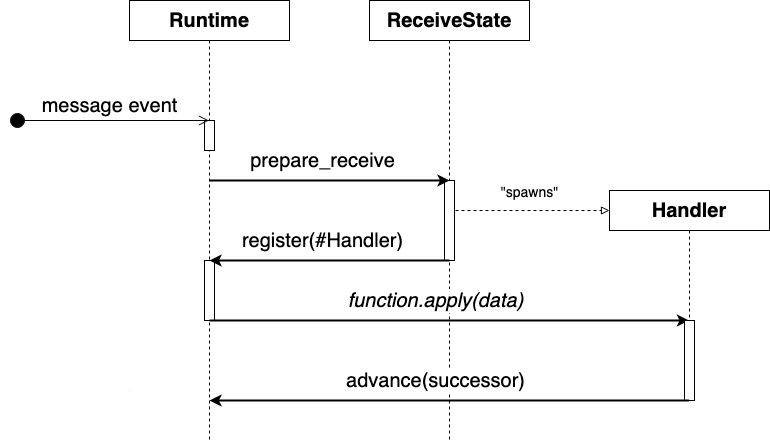
\includegraphics[width=\textwidth]{NodeRuntimeReceive2}
\caption{Message processed before transitioning to receive state}
\label{subfig:nodereceivemsgfirst}
\end{subfigure}
\hfill
\begin{subfigure}[b]{0.8\textwidth}
\centering
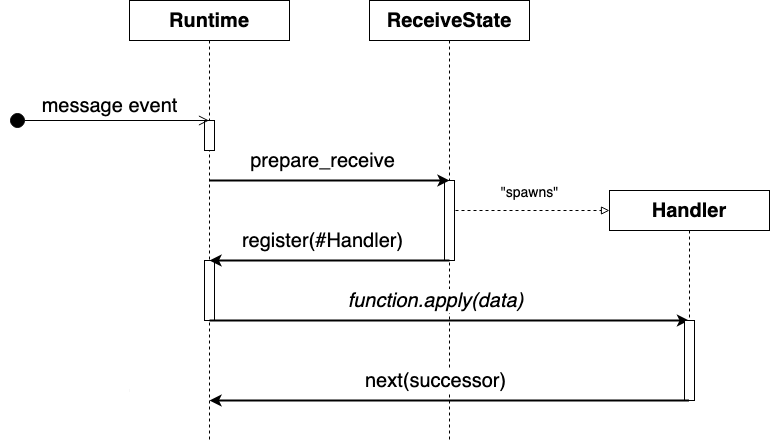
\includegraphics[width=\textwidth]{NodeRuntimeReceive1}
\caption{Message processed after transitioning to receive state}
\label{subfig:nodereceivehandlefirst}
\end{subfigure}
\caption{Possible Orderings for Handling Message Event and Preparing
Receive State}
\label{fig:nodereceivecompare}
\end{figure}

We observe that defining the handler using an optional type
is insufficient. We need a similar mechanism for handling messages
waiting for handlers, and we cannot assume an ordering on the arrival
of messages that are not causally related.

We proceed to generalise our approach from one optional-type
handler to two mappings:
\textbf{(1)} a mapping from endpoint to message queues\footnote{
TypeScript arrays have built-in $O(1)$ time complexity
\texttt{shift()} and \texttt{push()} operations, which
can be used as a queue.}, and
\textbf{(2)} a mapping from endpoint to handler queues.
To simply put, if an incoming message is waiting for its handler,
it gets enqueued in the message queue labelled by the sender of the message;
when the handler is created, it pops the message off the queue 
and directly processes it; the same logic applies for a handler waiting
for its message.
We could have used a mapping from endpoint to optional type,
but queue operations elegantly hides the mechanics of
\cref{line:callhandlerstart,line:callhandler2,line:callhandler}
in \cref{lst:noderuntimewsmsg}.

We outline the changes made to the \texttt{Session} class,
as shown in \cref{lst:nodesession}:

\begin{enumerate}
\item We construct types for these two mappings 
(\cref{line:mapped1,,line:mapped2}), 
using a generic mapped typed defined in
\cref{lst:noderolesmappedtypes}.

\item Empty queues are initialised for both mappings
(\cref{line:queue1,,line:queue2}).

\item Each endpoint has a different \texttt{onmessage}
event listener, which will interact with the message queue
and handler queue corresponding to that endpoint. 
We achieve this by changing the \texttt{receive()} method
to be parameterised on the role instead 
(\cref{line:receivefunc}),
so it \textit{generates} an event listener 
(\cref{line:receivefuncret})
tailored for receiving messages
from that particular role.

\item
The \texttt{register()} method now also takes the role
as a parameter (\cref{line:newregister}) in order to check the 
corresponding pair of queues.
\end{enumerate}

\begin{figure}[!h]
\begin{lstlisting}[language=javascript,tabsize=2]
type RoleToMessageQueue = Roles.PeersToMapped<any[]>; (*@\label{line:mapped1}@*)
type RoleToHandlerQueue = Roles.PeersToMapped<MessageHandler[]>; (*@\label{line:mapped2}@*)
type RoleToSocket = Roles.PeersToMapped<WebSocket>;

class Session {
	...
	private roleToSocket: RoleToSocket;
	private messageQueue: RoleToMessageQueue;
	private handlerQueue: RoleToHandlerQueue;
	
	constructor(...) {
		...
		Object.values(Roles.Peers).forEach(role => {
			const socket = this.roleToSocket[role];
			socket.onmessage = this.receive(role).bind(this);
		});
		
		this.messageQueue = { [Roles.Peers.Client]: [], }; (*@\label{line:queue1}@*)
		this.handlerQueue = { [Roles.Peers.Client]: [], }; (*@\label{line:queue2}@*)
		
		this.next(initialState);	
	}
	
	receive(from: Roles) { (*@\label{line:receivefunc}@*)
		return ({ data }) => { (*@\label{line:receivefuncret}@*)
			// Array.shift() can return undefined if empty
			const handler = this.handlerQueue[from].shift();
			if (handler !== undefined) {
				handler(data);
			} else {
				this.messageQueue[from].push(data);			
			}
		}
	}
	
	register(from: Roles.Peers, handler: MessageHandler) { (*@\label{line:newregister}@*)
		const message = this.messageQueue[from].shift();
		if (message !== undefined) {
			handler(message);		
		} else {
			this.handlerQueue[from].push(data);		
		}
	}
}
\end{lstlisting}
\captionof{lstlisting}{Modified \texttt{Session} class to correctly
handle message receive events}
\label{lst:nodesession}
\end{figure}

\begin{figure}[!h]
\begin{lstlisting}[language=javascript]
// Inside the Roles namespace...
export type PeersToMapped<Value> = { [Role in Peers]: Value };
\end{lstlisting}
\captionof{lstlisting}{Generic Mapped Type for Roles}
\label{lst:noderolesmappedtypes}
\end{figure}

Each endpoint must have consistency between
its message queue and handler queue.
We get the consistency from the simple fact that Node.js 
is a single-threaded runtime and execution is never pre-empted,
so there is no need to worry about atomic queue operations or
locking data structures.

We walk through how this design addresses the problems
in the previous example.

\begin{example}[Revisiting ``out-of-order'' message receives]
Consider the same multiparty session specified by the global type

\[
A \to S: \text{\lstonelinejs{M1(string)}}. 
B \to S: \text{\lstonelinejs{M2(number)}}. \texttt{end} 
\]

We show that our modified implementation addresses the problem:

\begin{enumerate}
\item 
\trole{S} transitions to its initial state,
``receive \lstonelinejs{M1(string)} from \trole{A}''.
\textit{The message queue for \trole{A} is empty,}
so the receive handler for \tmsg{M1} is registered 
\textit{under the handler queue for \trole{A}.}

\item
\tmsg{M2} arrives at \trole{S}, so the \texttt{onmessage}
handler is queued.

\item
\tmsg{M1} arrives at \trole{S}, so the \texttt{onmessage} handler
is queued.

\item
The \texttt{onmessage} handler for \tmsg{M2} is executed.
\textit{The handler queue for \trole{B} is empty, 
so \tmsg{M2} is added to the message queue for \trole{B}}.

\item
The \texttt{onmessage} handler for \tmsg{M1} is executed.
\textit{The handler queue for \trole{A} is non-empty,
so the handler is popped off the front of the queue 
and processes \tmsg{M1}.}

\item
\trole{S} transitions to the successor state, 
``receive \lstonelinejs{M2(number)} from \trole{B}''.
\textit{The message for \trole{B} is non-empty,
so \tmsg{M2} is popped off the queue and 
processed by the handler.}
\end{enumerate}

This execution is free of communication mismatches.
\end{example}

\subsection{Handling Termination}
WebSocket connections should be closed when the session terminates,
and both the browser endpoint and the server endpoint are capable
of closing connection. As we generate code for both, we define
a convention that the browser endpoint will close 
the WebSocket connection,
so we do nothing for this state at \cref{lst:noderuntime}.